\chapter{State spaces}
\lecture{1}{7/10}

\begin{definition}
    A \textbf{state space} is a (possibility infinite) set of states.
\end{definition}

Artifical intelligence search is about searching a state space for a suitable state. In a global search, we have \textbf{initial states} and we can move to other states through \textbf{state transitions}. Each transistion has an associated \textbf{step cost} and we are trying to make our way to a \textbf{goal state}. In moving to these \textbf{goal states}, we are trying to minimising or maximise the total \textbf{step costs}.

In the case of our state space being infinite, we only record the states that we have visited. We can clearly not store the entire state space as we do not have infinite memory.

In a local search, we do not have \textbf{actions} or \textbf{goal states}, we have objective cost from states reachable from the initial state. We will return to this later in the course.

\begin{example}
    Let's take the 8-puzzle problem. We take a state as a particular tile configration. We can represent this state as any data structure we want, such as a tuple $x \in (0, 1, \ldots, 8)^9$ or a $3 \times 3$ matrix. We can represent state transistions as an ordered pair of states so that we can move from the first state to the second. So let $x, y \in (0, 1, \ldots, 8)^9$. Then $(x, y)$ is a state transitions that shows that you can move from state $x$ to state $y$. 
\end{example}

\begin{remark}
    The way we abstract the problem does not matter, it can be done in many different ways.
\end{remark}

\begin{example}
    Consider the travelling salesman problem with $n$ cities. We will follow two abstractions of this problem.
    \begin{enumerate}
        \item Let a state be a list of $i$ distinct cities where $0 \leq i \leq n$. We represent a state transition as an ordered pair of states. Our initial state is an empty list and our goal state is a list of all cities. The step-cost is just simply the distance between the two cities that are in the state transition.

        \item Let a state be a list containing each of the $n$ cities exactly once. We represent a state transition as an ordered pair of states where the first state is the same as the second state with two cities switched around.  Our initial state is an arbitrary state and our goal state is every state. The step-cost is the distance between the two cities plus the distance between the first city and the initial city.
    \end{enumerate}
    In this example we are contrasting building a solution up from the ground and adapting a solution to an optimum.
\end{example}

The way we set up our states and state transitions are done how and when we need them. There is a fundamental tension between how we represent states and state transistions versus the implementation cost of building them.

We must ensure that our abstraction for a real-world problem is such that they correspond, so a solution to our problem matches the real-world problem.

We also have a consideration in optimisation problems in knowing whether not we have a optimal path to a goal state. In some situations, we must settle for a non-optimal solution.

In summary, to formally describe a real-world problem:

\begin{enumerate}
    \item define a state space;
    \item specify an initial sate;
    \item specify goal states;
    \item specificy a set of rules to describe transistions (possibility via actions) between states; and
    \item estabilish a notion of cost.
\end{enumerate}

\begin{definition}[Global path-based search problem]
    We have six fundamental properities to a global path-based search problem:
    \begin{enumerate}
        \item an initial state;
        \item a description of possible actions via a transistion function $\phi$;
        \item a goal test (a function that determines whether a state is a goal state);
        \item a non-negative step-cost function $\sigma$;
        \item a solution to the problem; and
        \item an optimal solution
    \end{enumerate}
\end{definition}

We will return to a local state-based search problems later.

We can generate search trees. We start with a root-node, which corresponds to the initial state. Then we expand the tree out with all the state transitions from this initial state. We then continue expanding the tree out.  We have goal-nodes, which correspond to goal states. We can think of search trees as rolling out a state space. There exists a bijection between the walks in the state space and the paths in the search tree.

\begin{figure}
    \centering
    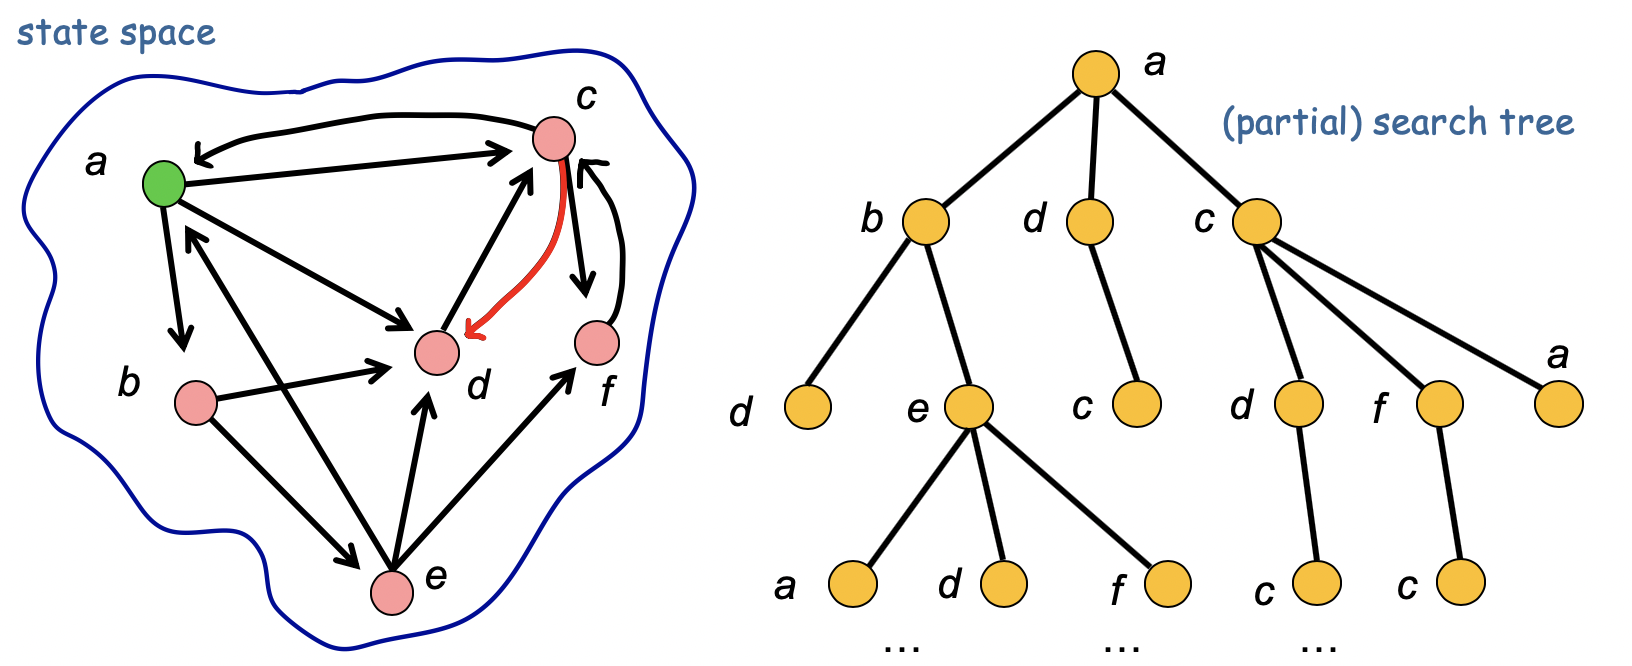
\includegraphics[width = 0.9\textwidth]{images/search-tree.png}
    \caption{State space to search tree diagram.}
    \label{fig:search-tree}
\end{figure}
